\chapter{Arhitektura i dizajn sustava}
            \noindent Arhitektura se može podijeliti na četiri podsustava:
            \begin{packed_item}
	
        	\item  Web poslužitelj
        	\item  Web aplikacija
        	\item  Baza podataka
            \item  Servis za autentifikaciju
            \end{packed_item}
            \\
            
\textit{Web preglednik} je program koji korisniku omogućuje pregled web-stranica i multimedijalnih sadržaja vezanih uz njih. Svaki internetski preglednik je prevoditelj. Dakle, stranica je pisana u kodu koji preglednik nakon toga interpretira kao nešto svakome razumljivo. Korisnik putem web preglednika šalje zahtjev web poslužitelju.
\begin{figure}[H]
	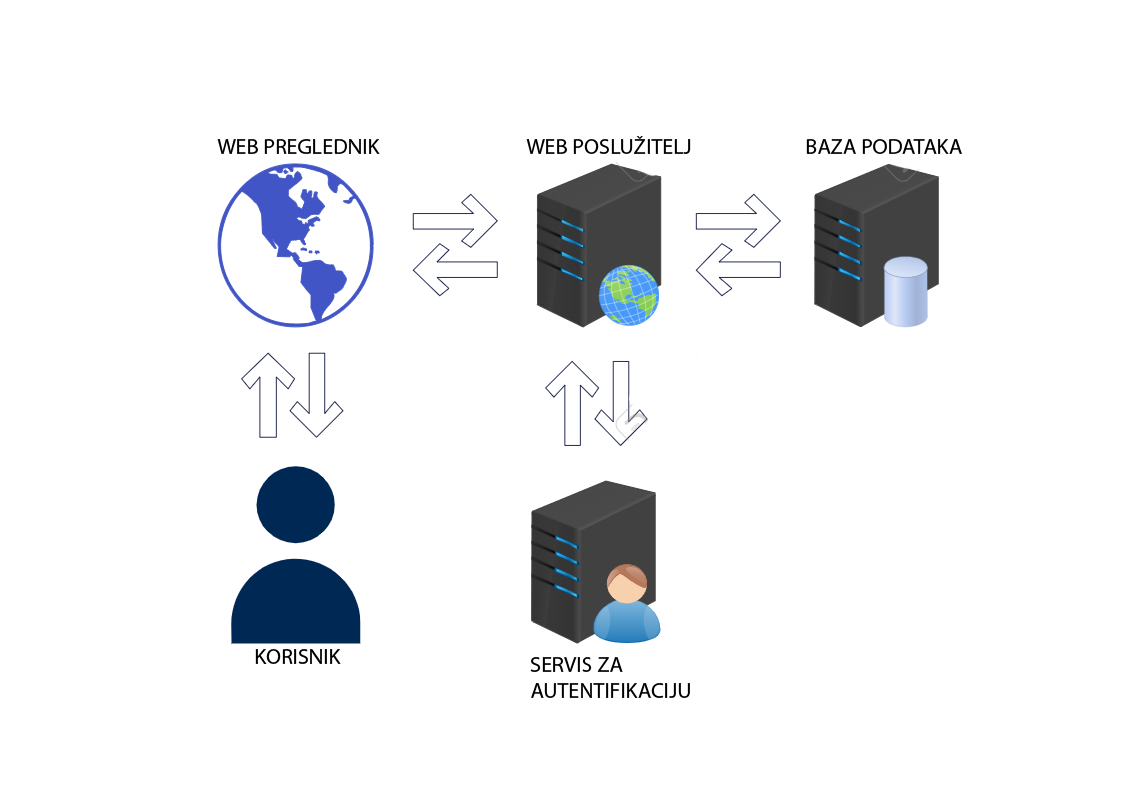
\includegraphics[scale=0.4]{slike/ArhitekturaSustava.png} 
	\centering
	\caption{Prikaz arhitekture}
	\label{fig:promjene}
\end{figure}

\newline
\\
\textit{Web poslužitelj} osnova je rada web aplikacije. Njegova primarna zadaća je komunikacija klijent s aplikacijom. Komunikacija se odvija preko HTTP (engl. \textit{Hyper Text Transfer Protocol}) protokola, što je protokol u prijenosu informacija na webu. Poslužitelj je onaj koji pokreće web aplikaciju te joj prosljeđuje zahtjeve.
\newline
\\
Korisnik korisi \textit{web aplikaciju} za obrađivanje željenih zahtjeva. Web aplikacija obrađuje zahtjev te ovisno o zahtjevu, pristupa bazi podataka i/ili servisu za autentifikaciju nakon čega preko poslužitelja vraća korisniku odgovor u obliku HTML dokumenta vidljivog u web pregledniku.
\newline
\\
Programski jezik kojeg smo odabrali za izradu naše web aplikacije je JavaScript za koji koristimo React biblioteku (engl. \textit{library}) te Next.js radni okvir (engl. \textit{framework}. Za autentifikaciju koristimo Google-ov modul za autentifikaciju iz njihovog servisa Firebase. Odabrano razvojno okruženje je Microsoft Visual Studio Code. Iako ne potpuno, arhitektura sustava temeljit će se na MVC (Model-View-Controller) konceptu. MVC koncept nije potpuno podržan od strane Next.js-a jer je to radni okvir koji omogućava posluživanje React aplikacija sa servera, a u samom React-u MVC koncept nije potpuno podržan. No, radi lakše izrade i organizacije projekta, odlučili smo na što bliži način implementirati MVC koncept.
\newline
\\
Karakteristika MVC koncepta je nezavisan razvoj pojedinih dijelova aplikaicje što za posljedicu ima jednostasvnije ispitivanje kao i jednostsavno razvijanje i dodavanje novih svojstava u sustav.
\newline
\\
MVC koncept sastoji se od:

\begin{packed_item}
	
        	\item  \textbf{Model} - Središnja komponenta sustava. Predstavlja dinamičke strukture podataka, neovisne o korisničkom sučelju. Izravno upravlja podacima, logikom i pravilima aplikacije. Također prima ulazne podatke od Controllera
        	\item \textbf{View} - Bilo kakav prikaz podataka, poput grafa. Mogući su različiti prikazi iste informacije poput grafičkog ili tabličnog prikaza podataka.
        	\item  \textbf{Controller} - Prima ulaze i prilagođava ih za prosljeđivanje Modelu i Viewu. Upravlja korisničkim zahtjevima i zemeljem njih izvodi daljnju interakciju s ostalim elementima sustava.
            \end{packed_item}


	
		

		

				
			\section{Baza podataka}

			Za potrebe našeg sustava koristit ćemo Firestore, Google-ovu NoSQL cloud bazu podataka iz njihovog servisa Firebase koja svojom strukturom omogućava lake izmijene koje će pratiti skaliranje aplikacije. Gradivna jedinka baze je kolekcija (engl. \textit{collection}) definirana svojim imenom i skupom dokumenata (engl. \textit{documents}). Zadaća baze podataka je brza i jednostavna pohrana, izmjena i dohvat podataka za daljnju obradu. Baza podataka ove aplikacije sastoji se od sljedećih kolekcija:
			\begin{packed_item}
			  
					  \item  users
					  \item  companies
					  \item  locations
					  \item  PaymentInfo
					  \end{packed_item}
				  
					  \subsection{Opis tablica}
					  
						  
						  
						  \textbf{Users}\hspace{1cm}  Ova tablica sadrži sve relevantne informacije za korisnike aplikacije. Sadrži atribute: UserId, Username, email i CompanyOwner(boolean atribut koji nam govori je li korisnik vlasnik obrta). Unutar sebe tablica sadrži kolekciju PaymentInfo u kojoj su informacije o kartičnom plaćanju. Tablica je u vezi \textit{One-to-One} s tablicom Companies i u vezi \textit{One-to-Many} je s tablicom Locations. 
		  
						  
						  \begin{longtblr}[
							  label=none,
							  entry=none
							  ]{
								  width = \textwidth,
								  colspec={|X[7,l]|X[6, l]|X[20, l]|}, 
								  rowhead = 1,
							  } %definicija širine tablice, širine stupaca, poravnanje i broja redaka naslova tablice
							  \hline {\textbf{Users}}	 \\ \hline[3pt]
							  \SetCell{LightGreen}UserId & VARCHAR	&  	Hashirani string jedinstven za svakog korisnika  	\\ \hline
							  Username	& VARCHAR & Nadimak pod kojim će se korisnik predstavljati u aplikaciji  	\\ \hline 
							  email & VARCHAR &  E-mail adresa korisnika \\ \hline 
							  CompanyOwner & BOOLEAN	&  True ako je korisnik vlasnik obrta, inače False		\\ \hline  
							  PaymentInfo & COLLECTION	&  Kolekcija s informacijama u plačanju		\\ \hline  
						  \end{longtblr}
		  
						  \textbf{PaymentInfo}\hspace{1cm} ova tablica(kolekcija) je sadržana unutar tablice Users. Ovakav način rada nam dopuštaju NoSql baze poput Firebasea. Unutar ove kolekcije nalaze se svi potrebni podatci o plačanju karticom. 
						  \begin{longtblr}[
							  label=none,
							  entry=none
							  ]{
								  width = \textwidth,
								  colspec={|X[9,l]|X[6, l]|X[20, l]|}, 
								  rowhead = 1,
							  } %definicija širine tablice, širine stupaca, poravnanje i broja redaka naslova tablice
							  \SetCell{LightGreen}\hline {\textbf{PaymentInfo}}	 \\ \hline[3pt]
							  VAT & INT	&  	Identifikacijski broj  	\\ \hline
							  Adress	& VARCHAR & Adresa vlasnika kartice  	\\ \hline 
							  CardCVC & INT &  Verifikacijski broj kartice \\ \hline 
							  ExpiryDate & DATE	&  Datum isteka kartice	\\ \hline  
							  City & VARCHAR	&  Grad vlasnika	\\ \hline  
							  CompanyNamePay & VARCHAR	&  Ime vlasnika kartice	\\ \hline 
							  CompanyOIBPay & VARCHAR	&  OIB vlasnika kartice	\\ \hline 
							  Country & VARCHAR	&  Zemlja vlasnika 	\\ \hline
							  FirstName & VARCHAR	&  Ime vlasnika 	\\ \hline 
							  LastName & VARCHAR	&  Prezime vlasnika	\\ \hline 
							  Region & VARCHAR	&  Regija vlasnika	\\ \hline
							  ZipCode & INT	&  Poštarski broj	\\ \hline 
							  Geopoint & GEOPOINT	&  Lokacija vlasnika kartice	\\ \hline 
							  
						  \end{longtblr}
							  
						  \textbf{Locations} \hspace{1cm} Ova tablica sadrži informacije o lokacijama dodanih od strane korisnika. Sadrži atribute: Ime lokacije, id korisnika koji je dodao lokaciju, status prikladnosti i koordinate. U vezi  \textit{Many-to-One} je s tablicom Users.
						  \begin{longtblr}[
							  label=none,
							  entry=none
							  ]{
								  width = \textwidth,
								  colspec={|X[6,l]|X[6, l]|X[20, l]|}, 
								  rowhead = 1,
							  } %definicija širine tablice, širine stupaca, poravnanje i broja redaka naslova tablice
							  \hline {\textbf{Locations}}	 \\ \hline[3pt]
							  \SetCell{LightGreen}Name & VARCHAR	&  Ime lokacije  	\\ \hline
							  \SetCell{LightBlue} UserId	& VARCHAR &  Hashirani string niz jedinstven za korisnika koji je dodao lokaciju 	\\ \hline  
							  Coordinates & VARCHAR &  Koordinate lokacije \\ \hline 
							  Category & VARCHAR &  Kategorija lokacije \\ \hline 
							  Upvotes & INT &  Broj pozitivnih ocjena \\ \hline 
							  Downvotes & INT &  Broj negativnih ocjena \\ \hline 
						  \end{longtblr}
						  \textbf{Companies} \hspace{1cm} Ova tablica sadrži informacije o dodanim obrtima. Posjeduje atribute: OIB obrta, Id vlasnika obrta, adresu, naziv obrta, kojoj kategoriji pripada i kratki opis obrta.  U vezi  \textit{One-to-One} je s tablicom Users.
						  \begin{longtblr}[
							  label=none,
							  entry=none
							  ]{
								  width = \textwidth,
								  colspec={|X[6,l]|X[6, l]|X[20, l]|}, 
								  rowhead = 1,
							  } %definicija širine tablice, širine stupaca, poravnanje i broja redaka naslova tablice
							  \hline {\textbf{Companies}}	 \\ \hline[3pt]
							  \SetCell{LightGreen}OIB & VARCHAR	&  Niz od 11 znamenki karakterističan za tu pravnu osobu  	\\ \hline
							  \SetCell{LightBlue} OwnerId	& VARCHAR &  Hashirani string niz jedinstven za korisnika koji je ujedino i vlasnik obrta 	\\ \hline  
							  Adress & VARCHAR	&  Adresa obrta	\\ \hline 
							  Name & VARCHAR &  Ime obrta \\ \hline 
							  Type & VARCHAR &  Kategorija kojoj obrt pripada \\ \hline 
							  Phone & VARCHAR &  Kontakt broj obrta\\ \hline 
							  Description & VARCHAR &  Kratki opis obrta \\ \hline 
							  Coordinates & GEOPOINT &  Koordinate obrta \\ \hline 
						  \end{longtblr}
		  
						  
						  
						  
					  
					  \subsection{Dijagram baze podataka}
						  %\textit{ U ovom potpoglavlju potrebno je umetnuti dijagram baze podataka. Primarni i strani ključevi moraju biti označeni, a tablice povezane. Bazu podataka je potrebno normalizirati. Podsjetite se kolegija "Baze podataka".}
						  %oznaci kljuceve
						  Na dijagramu ključevi su "boldani", a strani ključevi podcrtani.
						  \begin{figure}[H]
					  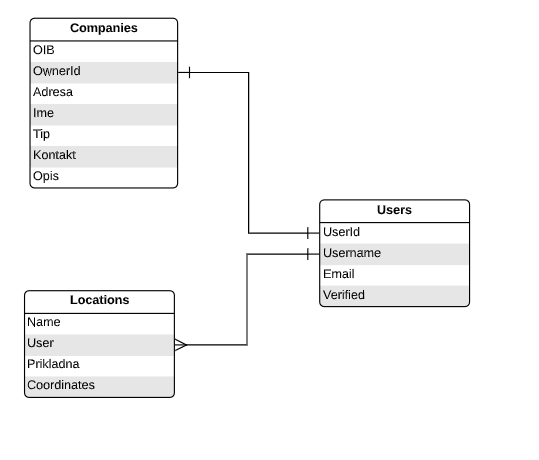
\includegraphics[scale=0.9]{slike/Baza.png}
					  \centering
					  \caption{Dijagram baze podataka}
					  \label{fig:promjene}
							\end{figure}
					  
			
		\section{Dijagram razreda}
		
			
			
			Na slici 4.3 prikazan je dijagram razreda cijelog projekta. Implementirane metode direktno komuniciraju s bazom podataka te vraćaju tražene podatke.
			
			PrivatnaForm služi za unos informacija o privatnom korisniku, vrši provjeru ispravnosti unosa i ako je sve u redu kreira korisnika u firebaseu
			
			VlasnikForm služi za unos informacija o obrtu. Sadrži podatke potrebne za neki obrt, provjerava ispravnost unesenih podataka i ako je sve u redu kreira korisnika u firebaseu.
	
	        Firebase služi za konfiguraciju baze i komunikaciju s istom. 
	        
	        Context stvara kontekst za trenutnog korisnika
	        
	        Hooks provjerava nalazi li se lozinka u "password blacklisti" i ako da, traži promjenu lozinke.

            Index prikazuje početnu stranicu na kojoj se prikazuje mapa, te sa koje se može prebaciti na ostale stranice.
            
	        Login korisniku prikazuje stranicu za ulogiravanje u aplikaciju. Prilikom log-ina gleda se postoji li korisnik u bazi, ako ne javlja se greška. Ako postoji ulogirava se u aplikaciju. Ne dozvoljava se upis dok sva polja nisu ispravno upisana.
	        
	        Register korisniku prikazuje stranicu za registraciju. U zavisnisti od odabranog prikazuje se ili "PrivatnaForma" ili "VlasnikForma"
	        
	        UserInfo prikazuje stranicu sa podatcima o ulogiranom korisniku. Prvotno funkcija povlači podatke o korisniku iz baze i ako je korisnik vlasnik firme, povlači i podatke o firmi. Te se isti podatci prikazuju na stranici

            
         
	        \begin{figure}[H]
			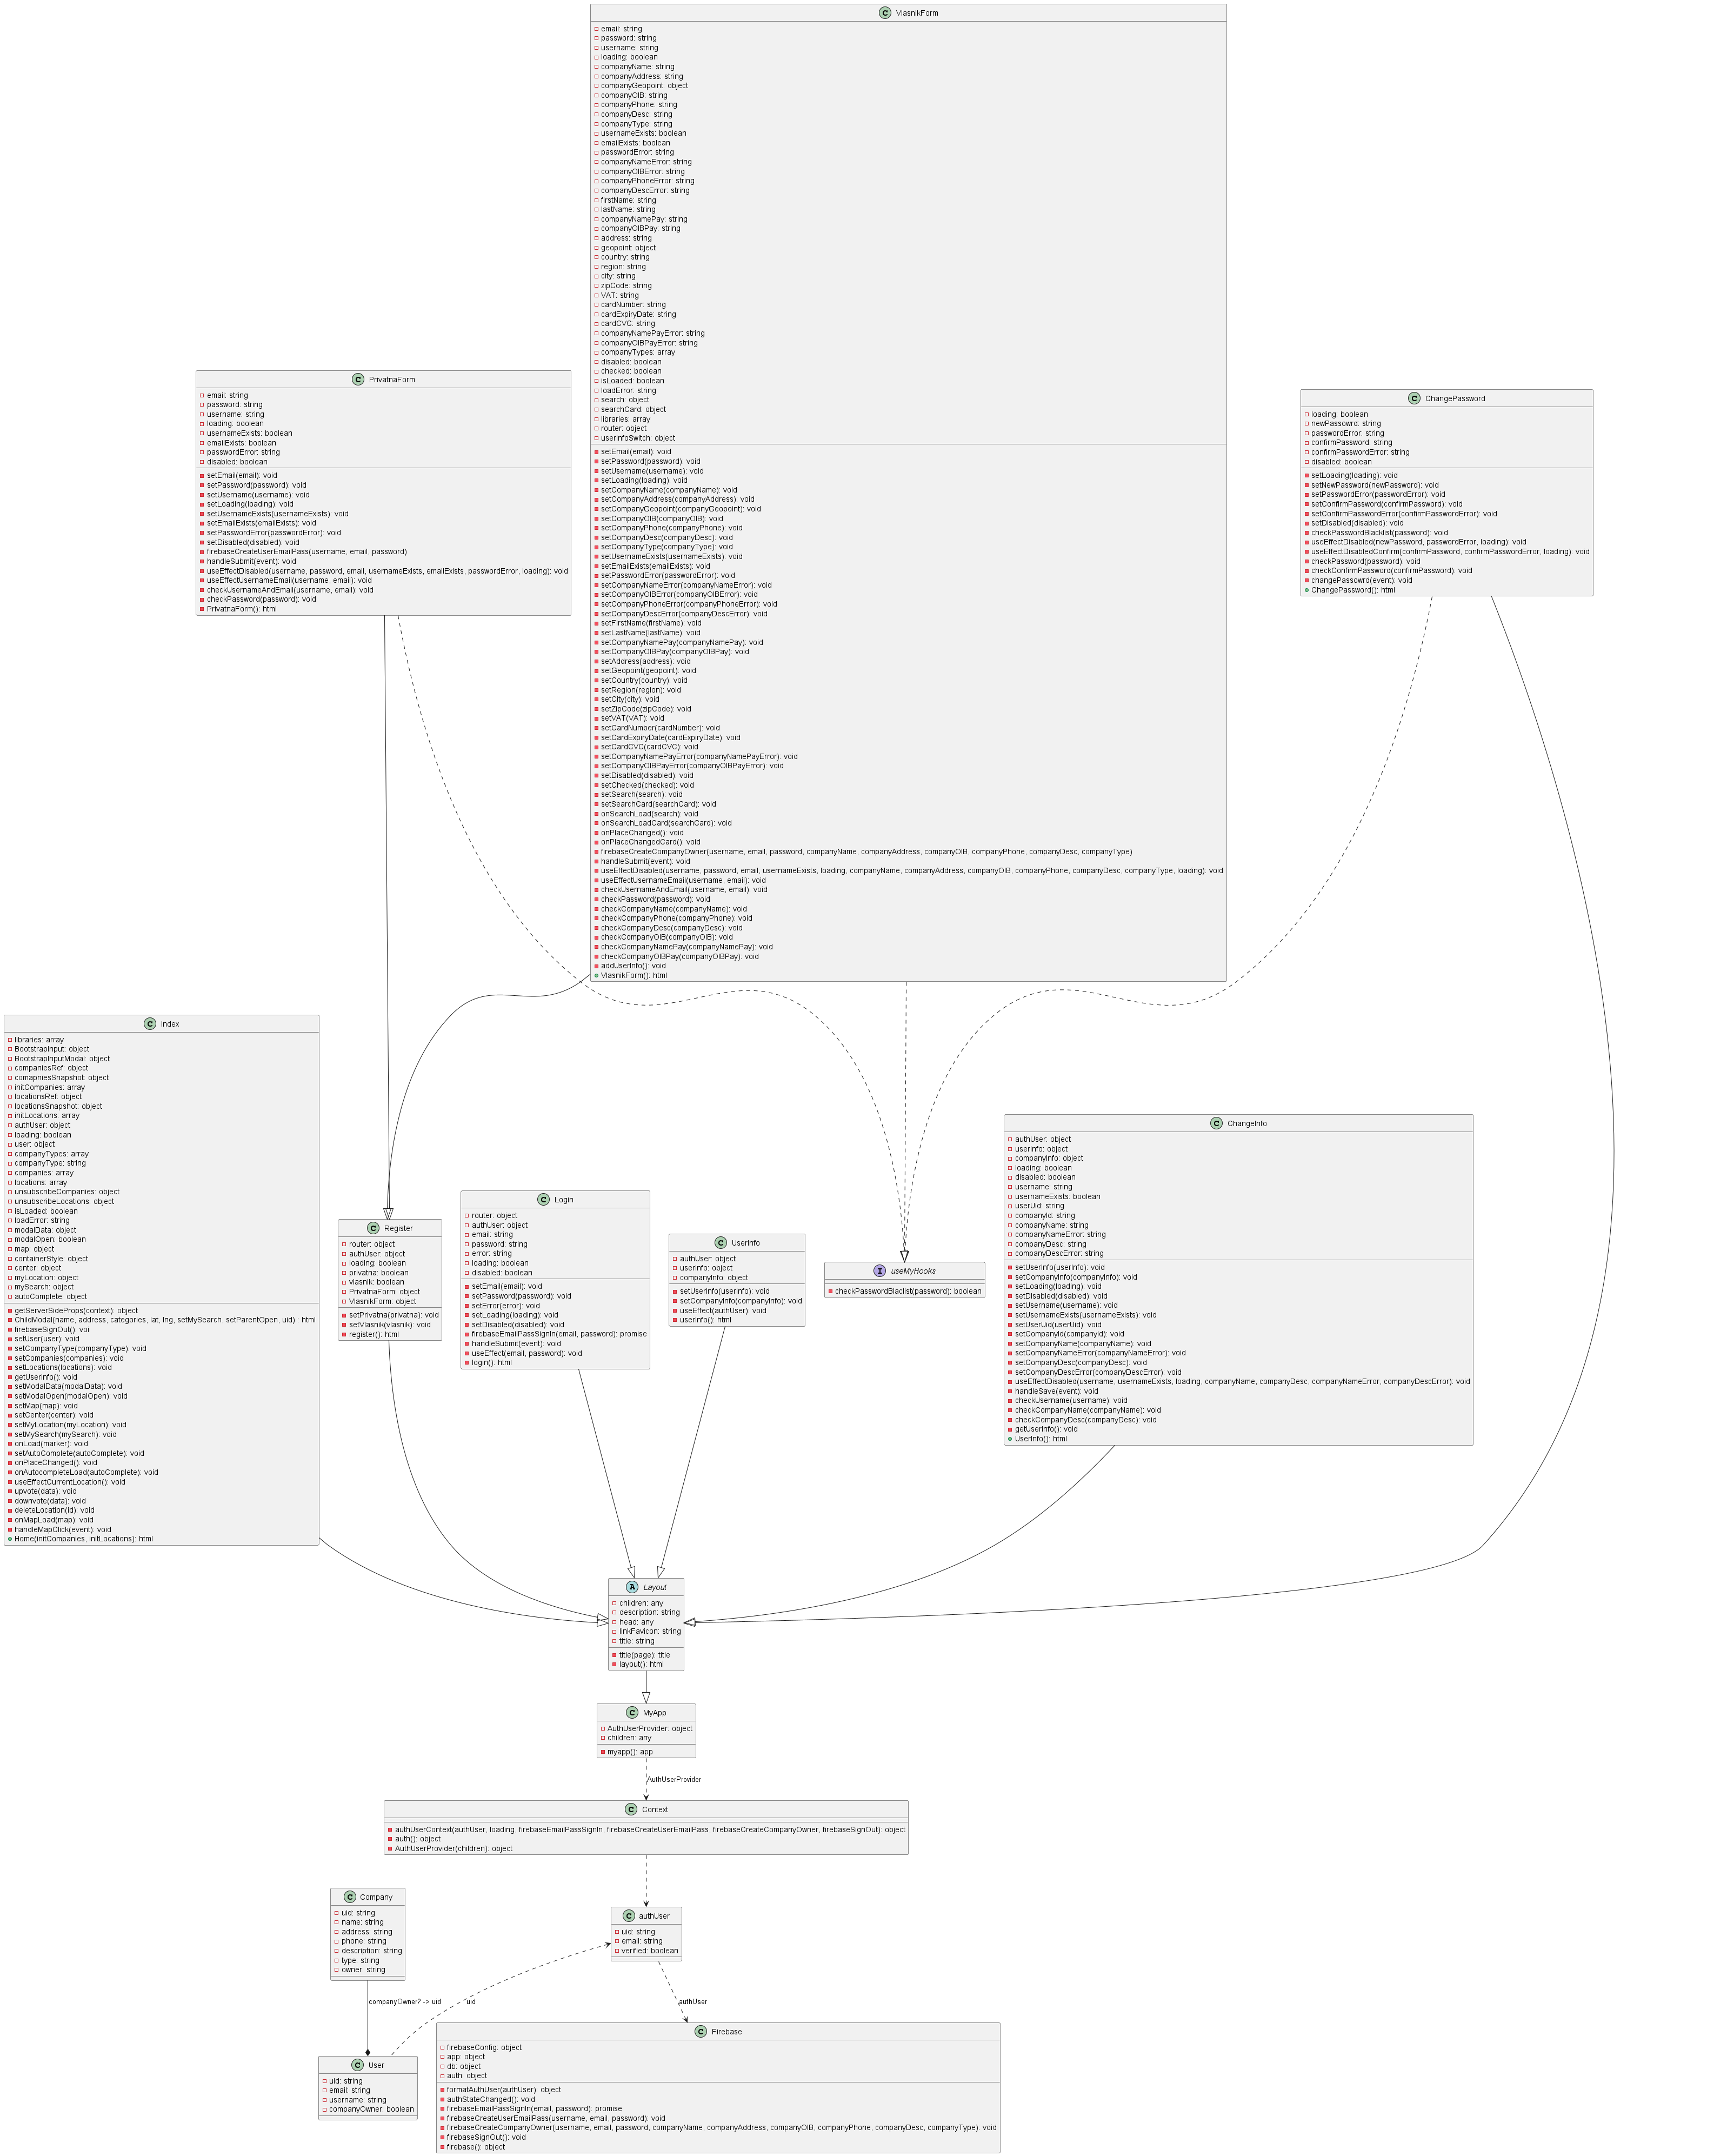
\includegraphics[scale=0.2]{slike/DijagramRazreda.png}
			\centering
			\caption{Dijagram razreda}
			\label{fig:promjene}
		          \end{figure}
            
			\section{Dijagram stanja}

           Dijagram stanja prikazuje stanje objekta te prijelaze iz jednog stanja u drugo temeljenje na događajima. Na slici 4.4 prikazan je dijagram stanja za registriranog korisnika. Nakon prijave, klijentu se prikazuje početna stranica na kojoj vidi kartu, te lokacije. Za odabranu lokaciju, korisnik može ostaviti ocjenu prikladnosti ako je lokacija postojeća, ili dodati novu ako ne postoji u bazi. Također, korisnik može pristupiti kartici Osobni podatci gdje može vidjeti i  uređivati osobne podatke, te obrisati račun ili dodatnu lokaciju. 

			\begin{figure}[H]
			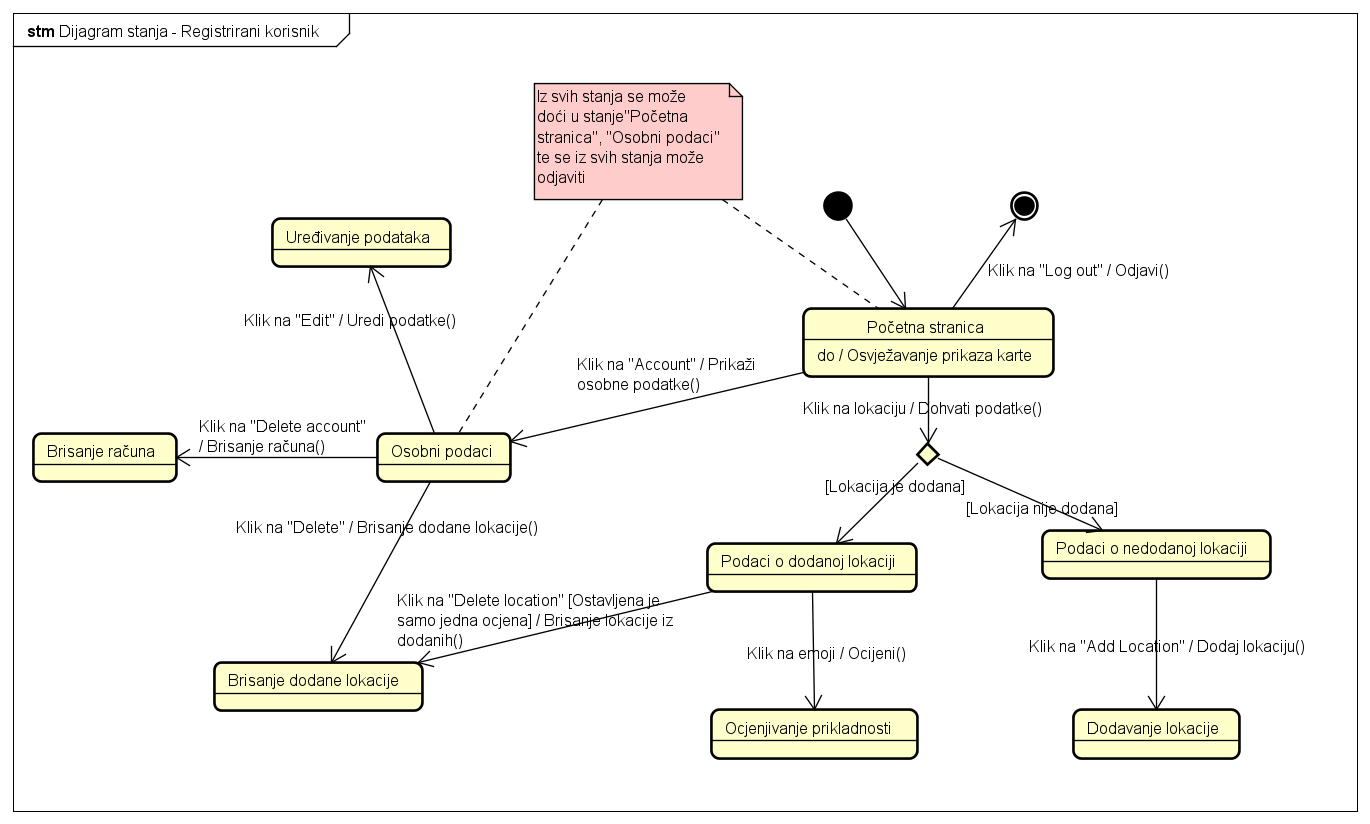
\includegraphics[scale=0.4]{slike/DijagramStanja.png}
			\centering
			\caption{Dijagram stanja}
			\label{fig:promjene}
				\end{figure}

         \section{Dijagram aktivnosti}
         
            Dijagram aktivnosti primjenjuje se za opis modela toka upravljanja ili toka podataka. Ne upotrebljava se za modeliranje događajima poticanog ponašanja. U modeliranju toka upravljanja svaki novi korak poduzima se nakon završenog prethodnog, a naglasak je na jednostavnosti. Na dijagramu akticnosti 4.5 prikazan je proces dodavanja lokacije. Korisnik se prijavljuje u sustav, odabire lokaciju na karti koja već nije u bazi podataka, te ispunjava podatke za lokaciju i dodaje je u bazu. 
         
			
			\begin{figure}[H]
			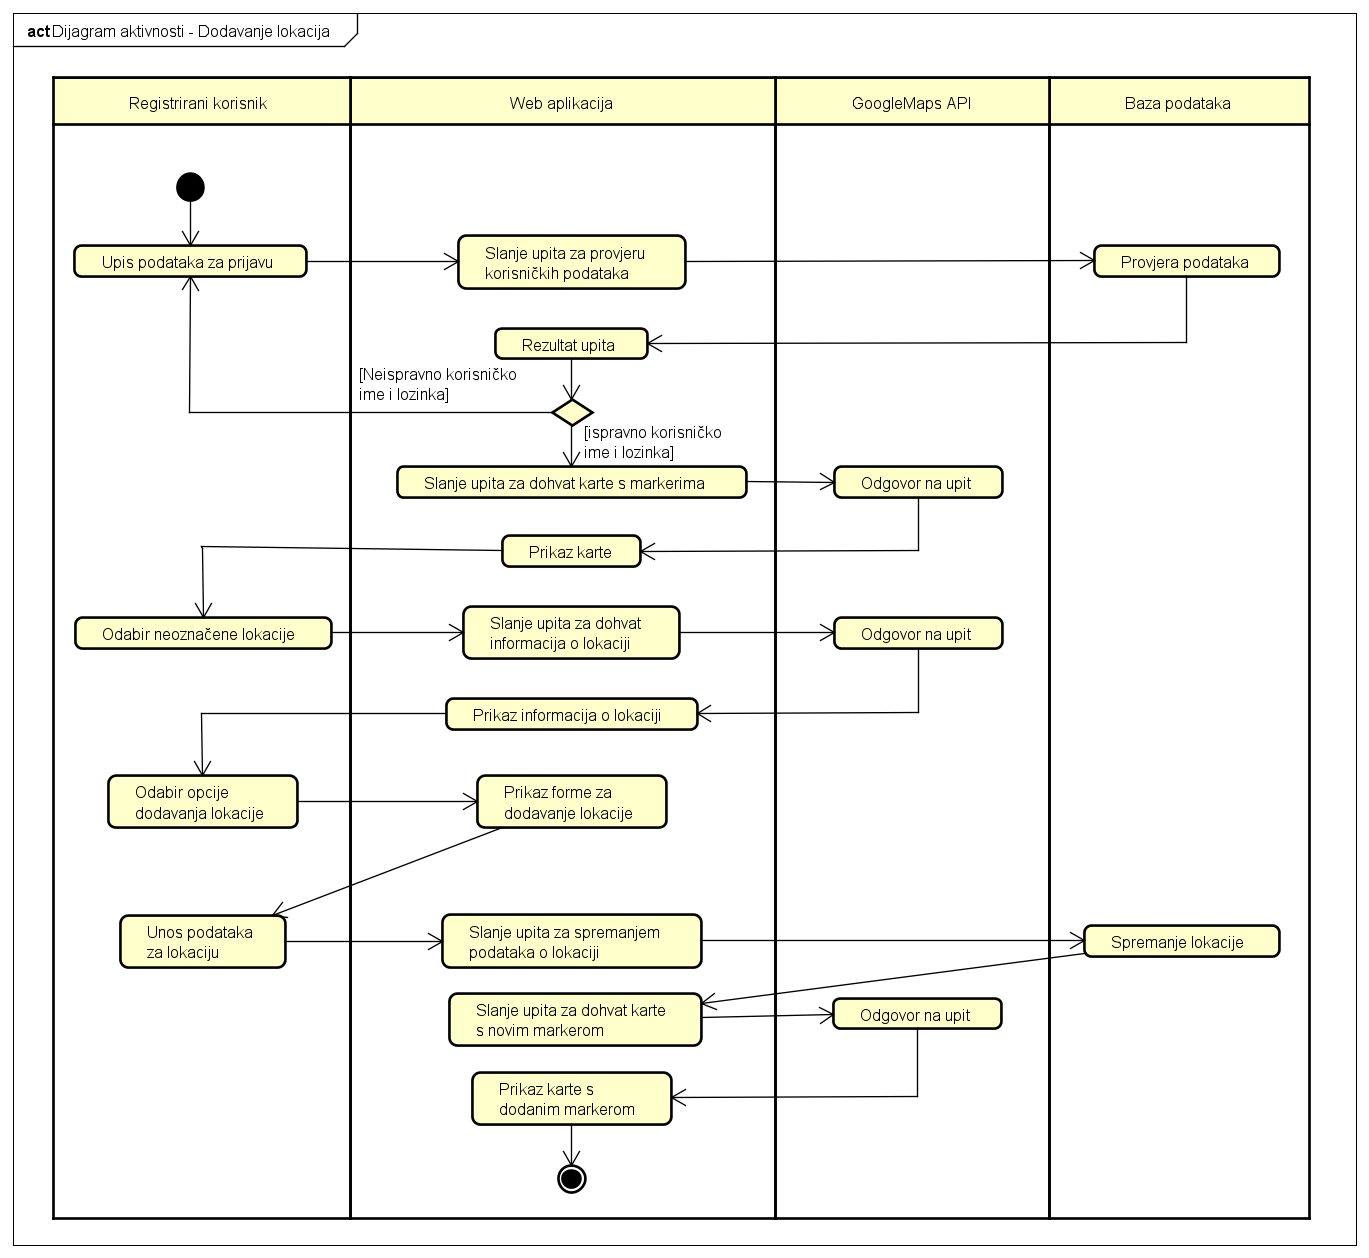
\includegraphics[scale=0.4]{slike/DijagramAktivnosti.png}
			\centering
			\caption{Dijagram aktivnosti}
			\label{fig:promjene}
				\end{figure}

            \section{Dijagram komponenti}

            Dijagram komponenti prikazan na slici 4.6. opisuje organizaciju i međuovisnost komponenti, interne strukture i odnose prema okolini. Sustavu se pristupa preko dva različita sučelja. Preko sučelja za dohvat HTML, CSS i JS datoteka poslužuju se datoteke koje pripadaju frontende dijelu aplikacije. Router je komponenta koja na upis s url određuje koja datoteka će se poslužiti na sučelje. Frontend dio se sastoji od niza
    
            
			%\textbf{\textit{dio 2. revizije}}\\			
			
			%\textit{Prilikom druge predaje projekta dijagram razreda i opisi moraju odgovarati stvarnom stanju implementacije}
			
			
			
			%\eject
		
		%\section{Dijagram stanja}
			
			
			%\textbf{\textit{dio 2. revizije}}\\
			
			%\textit{Potrebno je priložiti dijagram stanja i opisati ga. Dovoljan je jedan dijagram stanja koji prikazuje \textbf{značajan dio funkcionalnosti} sustava. Na primjer, stanja korisničkog sučelja i tijek korištenja neke ključne funkcionalnosti jesu značajan dio sustava, a registracija i prijava nisu. }
			
			
			%\eject 
		
		%\section{Dijagram aktivnosti}
			
			%\textbf{\textit{dio 2. revizije}}\\
			
			% \textit{Potrebno je priložiti dijagram aktivnosti s pripadajućim opisom. Dijagram aktivnosti treba prikazivati značajan dio sustava.}
			
			%\eject
		%\section{Dijagram komponenti}
		
			%\textbf{\textit{dio 2. revizije}}\\
		
			 %\textit{Potrebno je priložiti dijagram komponenti s pripadajućim opisom. Dijagram komponenti treba prikazivati strukturu cijele aplikacije.}